\subsection{EDA}

EDA provides an overview of what could be done to the data to improve the models' performance. 

\subsubsection{Data Profiling and Malformed Entries}

All of the columns and their data types can be seen at table \ref{tab:columns}. When checking for null values, all other columns are free from it other than \texttt{Income}. Upon inspection, there seems to be no connection with all the other attributes of the entries with null valued `Income`. As far as inspection and analysis goes, they seem to just be malformed entries. 

\texttt{Marital\_Status} also has multiple entries that could be thought of as different, similar, or sometimes even a malformed entry. In the list of unique values for the column, the values are \texttt{Divorced, Single, Married, Together, Widow, YOLO, Alone, Absurd}. Upon listing the value counts, \texttt{Alone, YOLO, Absurd} have very few entries which could be considered as outliers. There are been thoughts of merging some of these entries to the other entries with bigger value counts; e.g. \texttt{Single} would adopt the records with \texttt{Alone}, etc. However the problem lies wherein there is no way to deduce their backgrounds and whether or not the adopting categories should take in the outliers. To further explain, there is no way to tell if a record that is \texttt{Alone} might have came from a divorced background or if they simply are single. However further explanation of the choice between data integrity and model performance would come in later in experimentations

\subsubsection{Univariate Analysis}

The skew and imbalance of data attributes can be seen upon further isolated inspection. Firstly, \texttt{Income}'s central tendencies at table \ref{tab:income desc}

\begin{table}[H]
    \caption{Income column's descriptive statistics}
    \label{tab:income desc}
    \centering
    \begin{tabularx}{0.5\linewidth}{l>{\raggedleft\arraybackslash}X}
        \toprule
        count & 2216 \\
        mean & 52247.251354\\
        std & 25173.076661\\
        min & 1730\\
        25\% & 35303\\
        50\% & 51381.5\\
        75\% & 68522\\
        max & 666666\\
        \bottomrule
    \end{tabularx}
\end{table}

To put into perspective figure \ref{fig:income hist} shows the distance of the max value from the mean of the distribution with a skewness of 6.763487372811116

\begin{figure}[H]
    \centering
    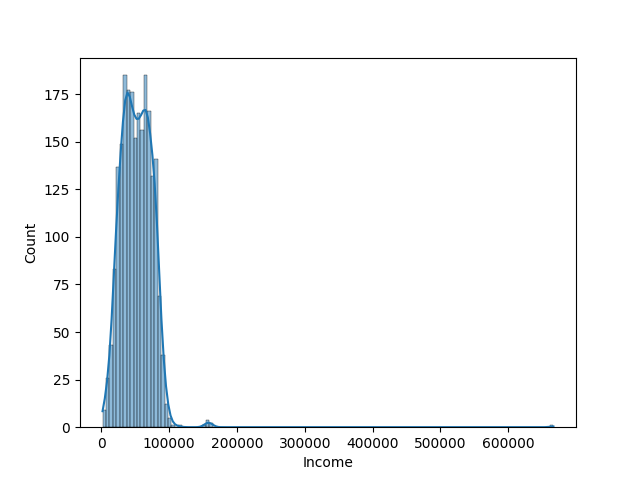
\includegraphics[width=\linewidth]{figures/income_histplot.png}
    \caption{histogram of Income values}
    \label{fig:income hist}
\end{figure}

Depending if the models are robust to outliers, they will be removed, experimentations will further explain these phenomena

\texttt{Education}'s entries are listed at figure \ref{fig:educ bar}. While it could be considered that the \texttt{Basic} records are outliers, removing them may misrepresent the dataset.

\begin{figure}[H]
    \centering
    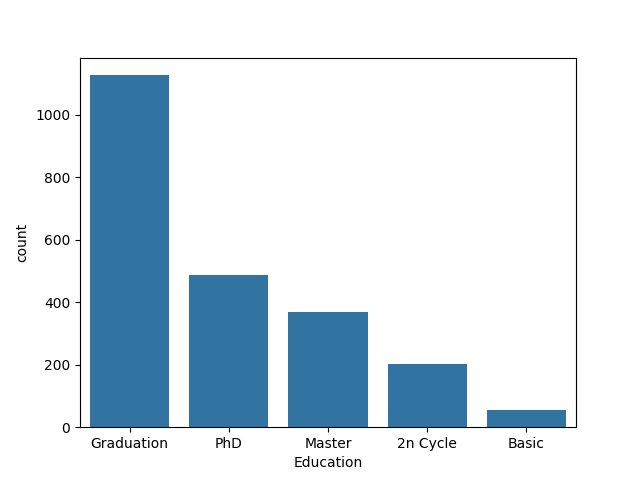
\includegraphics[width=\linewidth]{figures/education_barplot.png}
    \caption{Bar plot of value counts of the Education column}
    \label{fig:educ bar}
\end{figure}


